\documentclass[a4paper]{article}
\usepackage[14pt]{extsizes} 
\usepackage[T2A]{fontenc}
\usepackage[utf8]{inputenc}
\usepackage{natbib}
\usepackage{graphicx}
\usepackage{amsmath}
\usepackage[english]{babel}
\usepackage{fontspec}
\usepackage{amsmath,amsfonts,amssymb,amsthm,mathtools,mathrsfs}
\usepackage{icomma}
\usepackage{fullpage}
\usepackage{ulem}
\usepackage{eufrak}
\usepackage{setspace}
\usepackage{listings}
\usepackage{indentfirst}
\usepackage[left=2cm,right=1.5cm,top=2cm,bottom=2cm]{geometry}
\usepackage{xcolor}
\usepackage{float}
\usepackage{csquotes}

\setmainfont[Ligatures={TeX,Historic}]{Times New Roman}
\setlength{\parindent}{5ex}
\setlength{\parskip}{1em}
\renewcommand{\baselinestretch}{1}

\graphicspath{{images/}}

\definecolor{buzzlightyear}{HTML}{8757A5}
\definecolor{grass}{HTML}{738D06}
\definecolor{literal}{HTML}{F18A2B}
\definecolor{commentcolor}{HTML}{8E908B}

\lstdefinestyle{habrstyle}{
    backgroundcolor=\color{white},   
    commentstyle=\color{commentcolor},
    keywordstyle=\bfseries\color{buzzlightyear},
    numberstyle=\tiny\color{commentcolor},
    stringstyle=\color{grass},
    basicstyle=\ttfamily\footnotesize,
    breakatwhitespace=false,         
    breaklines=true,                 
    captionpos=b,                    
    keepspaces=true,                 
    numbers=left,                    
    numbersep=5pt,                  
    showspaces=false,                
    showstringspaces=false,
    showtabs=false,                  
    tabsize=4
}

\lstset{style=habrstyle}

\begin{document}

    % FIRST PAGE
    \begin{center}
        \begin{center}
        \hfill \break
        \normalsize{Санкт-Петербургский государственный политехнический}\\
        \normalsize{университет Петра Великого}\\
        \hfill \break
        \normalsize{\textbf{Высшая школа интеллектуальных систем и}}\\ 
        \normalsize{\textbf{суперкомпьютерных технологий}}\\ 
        \hfill \break
        \hfill \break
        \hfill \break
        \normalsize{Лабораторная работа}\\
        \hfill \break
        \hfill \break
        \normalsize{\LARGE Шум}\\
        \end{center}
        \hfill \break
        \hfill \break
        \hfill \break
        \hfill \break
        \hfill \break
        \hfill \break
        \hfill \break
        \hfill \break
        \hfill \break
        \hfill \break
        \begin{flushright}
            \normalsize{Работу выполнил студент}\\
            \normalsize{3-го курса, группа 3530901/80201}\\
            \normalsize{Сахибгареев Рамис Ринатович}\\
            \hfill \break
            \normalsize{Преподаватель:}\\
            \normalsize{Богач Наталья Владимировна}\\
        \end{flushright}
        \hfill \break
        \hfill \break
        \hfill \break
        \hfill \break
        \begin{center} Санкт-Петербург 2021 \end{center}
        \thispagestyle{empty}
    \end{center}
    % FIRST PAGE [END]
    
    \newpage
        \tableofcontents
    
    \newpage
         \listoffigures
    
    \newpage
         \lstlistoflistings   
     
    % START START START START START
    \newpage
        \section{Part 1: Env sounds}
        
        In this part we need to explore how different real-life environment sounds looks like. To do it rain and sea sound was used.
        
        Firstly, let's check how overall spectrogram of sea looks like.
        \begin{lstlisting}[language=Python,caption=File load and spectrum plotting,label={lst:part1_1}]
    from thinkdsp import *
    wave = read_wave('data/sea.wav')
    spectrum = wave.make_spectrum()
    spectrum.plot()
        \end{lstlisting}
        \begin{figure}[H]
            \centering
            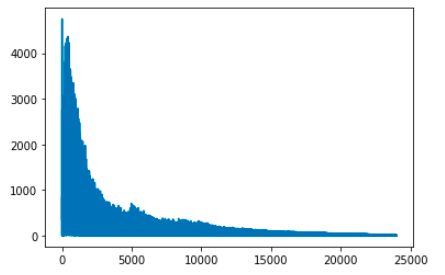
\includegraphics[width=\textwidth]{img/sea_overall.png}
            \caption{Sea overall spectrum}
            \label{fig:part1_1_1}
        \end{figure}
        
        To make it easier for researching let's plot powers in log-scaled axis. By dominance of lower pitches we can say, that it can be a pink or a red noise.
        \begin{lstlisting}[language=Python,caption=Log spectrum,label={lst:part1_2}]
    spectrum.plot_power()
    loglog = dict(xscale='log', yscale='log')
    decorate(xlabel='Frequency (Hz)', **loglog)
        \end{lstlisting}
        \begin{figure}[H]
            \centering
            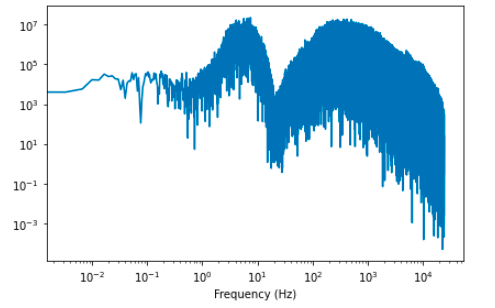
\includegraphics[width=\textwidth]{img/sea_overall_log.png}
            \caption{Sea overall log spectrum}
            \label{fig:part1_1_2}
        \end{figure}
        
        Secondly, let's check how signal changes over the time. To do it I've selected 2 segments and plotted an spectrum for them. We can see, that both segments look almost the same.
        \begin{lstlisting}[language=Python,caption=Segments spectrum,label={lst:part1_3}]
    seg1 = wave.segment(start=10, duration=2)
    seg2 = wave.segment(start=20, duration=2)
    spec1 = seg1.make_spectrum()
    spec2 = seg2.make_spectrum()
    spec2.plot(color='red')
    spec1.plot(color='blue')
        \end{lstlisting}
        \begin{figure}[H]
            \centering
            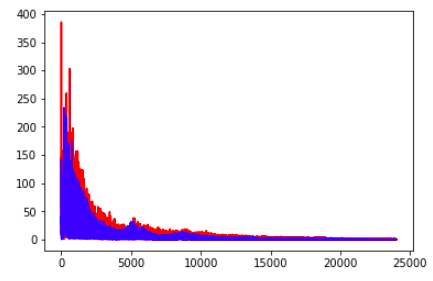
\includegraphics[width=\textwidth]{img/sea_seg.png}
            \caption{Sea segments log spectrum}
            \label{fig:part1_1_3}
        \end{figure}
        \begin{lstlisting}[language=Python,caption=Log spectrum of segments,label={lst:part1_4}]
    spec2.plot_power(color='red')
    spec1.plot_power(color='blue')
    loglog = dict(xscale='log', yscale='log')
    decorate(xlabel='Frequency (Hz)', **loglog)
        \end{lstlisting}
        \begin{figure}[H]
            \centering
            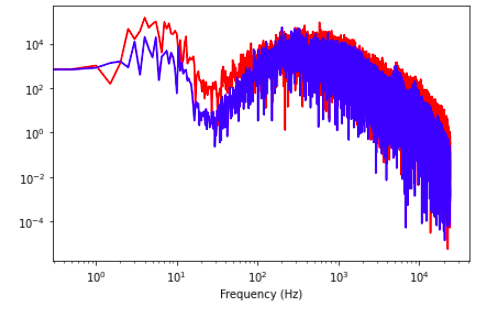
\includegraphics[width=\textwidth]{img/sea_seg_log.png}
            \caption{Sea segments spectrum}
            \label{fig:part1_1_4}
        \end{figure}
        
        To make sure, that signal is consistent over the time, let's plot a spectrogram of a signal. We can see, that signal stay almost the same with periodic spikes - crushing waves sound.
        \begin{lstlisting}[language=Python,caption=Overall spectrogram,label={lst:part1_5}]
    wave.make_spectrogram(2048).plot(high=5000)
    decorate(xlabel='Time(s)', ylabel='Frequency (Hz)')
        \end{lstlisting}
        \begin{figure}[H]
            \centering
            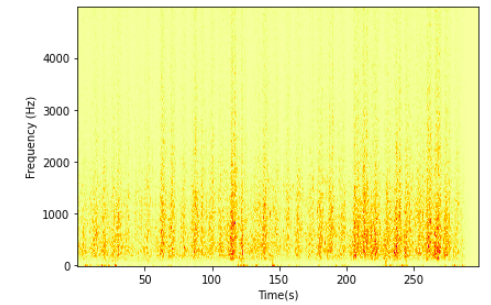
\includegraphics[width=\textwidth]{img/sea_spectrogram.png}
            \caption{Sea overall spectrogram}
            \label{fig:part1_1_5}
        \end{figure}
        
        Let's do the same to the other sound - sound of the rain. By looking on its overall spectrum we can say, that it is a pink or a red noise.
        \begin{figure}[H]
            \centering
            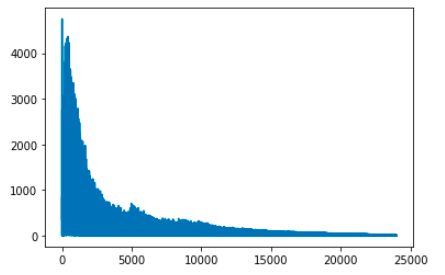
\includegraphics[width=\textwidth]{img/sea_overall.png}
            \caption{Rain overall spectrum}
            \label{fig:part1_2_1}
        \end{figure}
        \begin{figure}[H]
            \centering
            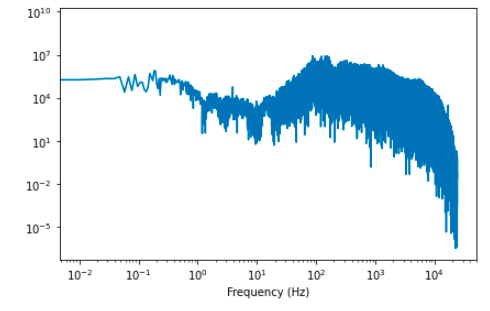
\includegraphics[width=\textwidth]{img/rain_overall_log.png}
            \caption{Rain overall log spectrum}
            \label{fig:part1_2_2}
        \end{figure}
        
        By checking its segments we can say, that signal stays consistent over the time.
        \begin{figure}[H]
            \centering
            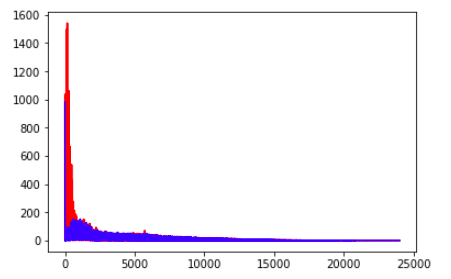
\includegraphics[width=\textwidth]{img/rain_seg.png}
            \caption{Rain segments log spectrum}
            \label{fig:part1_2_3}
        \end{figure}
        \begin{figure}[H]
            \centering
            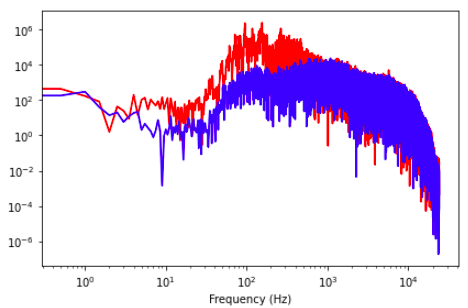
\includegraphics[width=\textwidth]{img/rain_seg_log.png}
            \caption{Rain segments spectrum}
            \label{fig:part1_2_4}
        \end{figure}
        
        However, by looking on the overall spectrogram we can say, that there was 2 loud events like something fell or hit something other.
        \begin{figure}[H]
            \centering
            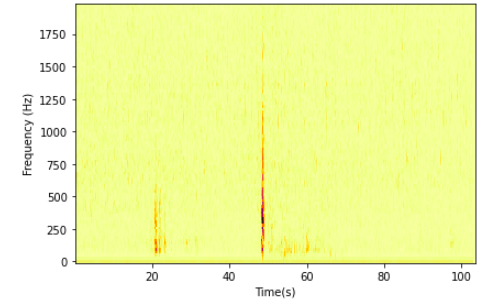
\includegraphics[width=\textwidth]{img/rain_spectrogram.png}
            \caption{Rain overall spectrogram}
            \label{fig:part1_2_5}
        \end{figure}
    
        A lot of environmental sounds has red/ping nature, and these sounds are not an exception.
    
    \newpage
        \section{Part 2: Barrett's method}

        In this part we need to create Berrett's method to estimate signal's power using its segments.
        
        Let's declare a function:
            
        \begin{lstlisting}[language=Python,caption={Barrett's function definition},label={lst:sawtooth_def}]
    def bartlett_method(wave, seg_length=512):
        spectro = wave.make_spectrogram(seg_length , True)
        spectrums = spectro.spec_map.values()
        pwrs = [spectrum.power for spectrum in spectrums]
        hs = np.sqrt(sum(pwrs) / len(pwrs))
        fs = next(iter(spectrums)).fs
        spectrum = Spectrum(hs, fs, wave.framerate)
        return spectrum
        \end{lstlisting}
        
        Next, let's check how it's work using segments from previous part:
            
        \begin{lstlisting}[language=Python,caption=Sawtooth wave plot code,label={lst:sawtooth_check}]
    p1 = bartlett_method(seg1)
    p2 = bartlett_method(seg2)
    p1.plot_power(color='blue')
    p2.plot_power(color='red')
    decorate(xlabel='Frequency (Hz)',ylabel='Power',**loglog)
        \end{lstlisting}

        \begin{figure}[H]
          \centering
          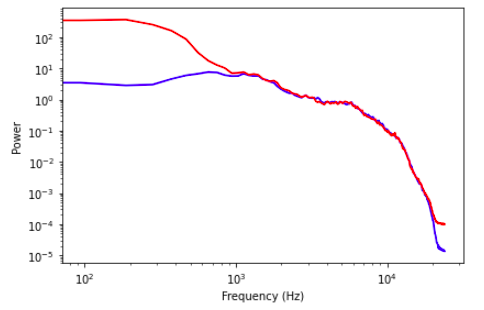
\includegraphics[width=\textwidth]{img/seg_barrett.png}
          \caption{Mean powers by Barrett's method}
          \label{fig:sawtooth_wave_plot}
        \end{figure}
            
        We can see how close these 2 graphs are. It happens because of noisy nature of the signal - mean energies of the segments represents mean energy of all signal.
        
    \newpage
        \section{Part 3: GREATEST CRYPTOCURRENCY OF ALL TIME (aka. bitcoin)}
            
        In this part we need to try to use wave analysis tools to the bitcoin chart.
        
        Let's read the bitcoin cost at the end of every day and represent it as a wave. 
        
        \begin{lstlisting}[language=Python,caption=Bitcoin to a wave,label={lst:als_sqr}]
    data = pd.read_csv('data/bitcoin.csv')
    price = data['Closing Price (USD)']
    count = data.index
    wave = Wave(price,count,framerate=1)
    wave.plot()
    decorate(xlabel='Day')
        \end{lstlisting}
            
        \begin{figure}[H]
            \centering
            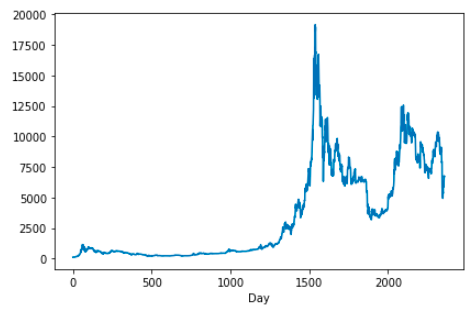
\includegraphics[width=\textwidth]{img/bitcoin_chart.png}
            \caption{Bitcoin chartt}
            \label{fig:als_sqr}
        \end{figure}
        
        Let's look, how looks a logarithmic graph of a spectrum's power.
        
        \begin{lstlisting}[language=Python,caption=Bitcoin to a spectrum's power,label={lst:als_sqr}]
    spectrum = wave.make_spectrum()
    spectrum.plot_power()
    decorate(**loglog)
    print(spectrum.estimate_slope()[0])
        \end{lstlisting}
        
        \begin{figure}[H]
            \centering
            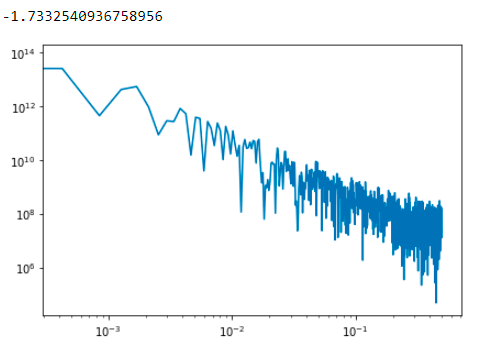
\includegraphics[width=\textwidth]{img/bitcoin_as_wave.png}
            \caption{Bitcoin as power}
            \label{fig:als_clr}
        \end{figure}
            
        As we can see, bitcoin acts like a pink or a brown noise. By checking its slope rate, that equals ti -1.73 we cannot be sure, what noise it is - red or brown.
            
    \newpage
        \section{Part 4: Geiger counter}
        
            In this part we need to explore Poisson distribution. To do it I've changed distribution function to \texttt{np.random.poisson}.
            
            Code of new noise is next. We can see on the plot, that it has 51 picks, when expected value is 50.
            
            \begin{lstlisting}[language=Python,caption=Usage of Poisson,label={lst:part4}]
    class UncorrelatedPoissonNoise(Noise):
        def evaluate(self, ts):
            ys = np.random.poisson(self.amp, len(ts))
            return ys
            
    signal = UncorrelatedPoissonNoise(amp=0.001)
    wave = signal.make_wave(duration=5, framerate=10000)
    wave.plot()
    print(sum(wave.ys))
            \end{lstlisting}
            
            \begin{figure}[H]
                \centering
                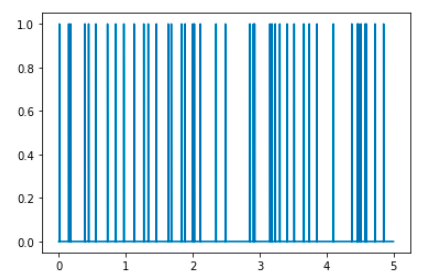
\includegraphics[width=\textwidth]{img/geiger.png}
                \caption{Waveform pf Poisson}
                \label{fig:part42}
            \end{figure}
            
            Let's create logarithmic power plot. We can see, that it is clear white noise.
            
            \begin{lstlisting}[language=Python,caption=Usage of Poisson,label={lst:part4}]
    spectrum = wave.make_spectrum()
    spectrum.plot_power()
    decorate(xlabel='Frequency (Hz)',**loglog)
    print(spectrum.estimate_slope()[0])
            \end{lstlisting}
            
            \begin{figure}[H]
                \centering
                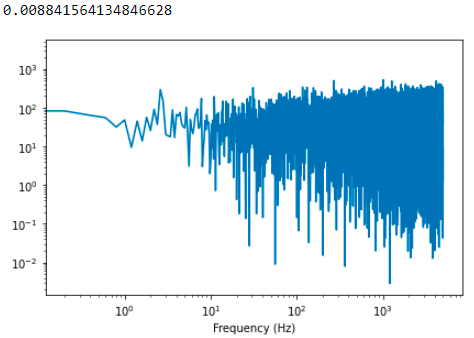
\includegraphics[width=\textwidth]{img/geiget_power.png}
                \caption{Geiger power plot}
                \label{fig:part42}
            \end{figure}
            
    \newpage
        \section{Part 5: Voss-McCartney algorithm}
        
            Algorithm, that creates a pink noise by cutting of higher frequencies is slow and ineffective, that's why new algorithms was created. One of them is Voss-McCartney algorithm.
            
            Code of the class - Listing \ref{lst:part5_1}
            
            \begin{lstlisting}[language=Python,caption=Voss-McCartney algorithm,label={lst:part5_1}]
    def voss(nrows , ncols=16):
        array = np.empty((nrows , ncols))
        array.fill(np.nan)
        array[0, :] = np.random.random(ncols)
        array[:, 0] = np.random.random(nrows)
        n = nrows
        cols = np.random.geometric(0.5, n)
        cols[cols >= ncols] = 0
        rows = np.random.randint(nrows , size=n)
        array[rows, cols] = np.random.random(n)
        df = pd.DataFrame(array)
        df.fillna(method='ffill', axis=0, inplace=True)
        total = df.sum(axis=1)
        return total.values
            \end{lstlisting}
            
            Let's create a wave and its plot using this pink-noise generator
            
            \begin{lstlisting}[language=Python,caption=Wave and plot creation,label={lst:part5_2}]
    wave = Wave(voss(10000))
    wave.unbias()
    wave.normalize()
    wave.plot()
            \end{lstlisting}
            
            \begin{figure}[H]
                \centering
                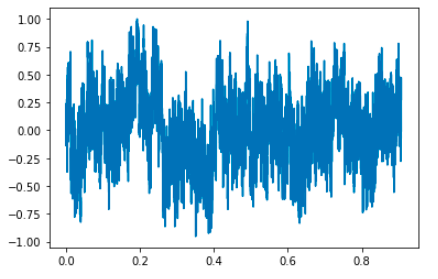
\includegraphics[width=\textwidth]{img/vvos.png}
                \caption{Resulting wave}
                \label{fig:part5_1}
            \end{figure}
            
            To be sure, that resulting noise is pink, lets build spectrum's power plot and calculate its slope. It is equals to -1.017 - the noise is pink.
            
            \begin{lstlisting}[language=Python,caption=Wave and plot creation,label={lst:part5_2}]
    spectrum = wave.make_spectrum()
    # don't break the math's laws
    spectrum.hs[0] = 0
    spectrum.plot_power()
    decorate(xlabel='Frequency (Hz)',**loglog)
    print(spectrum.estimate_slope()[0])
            \end{lstlisting}
            
            \begin{figure}[H]
                \centering
                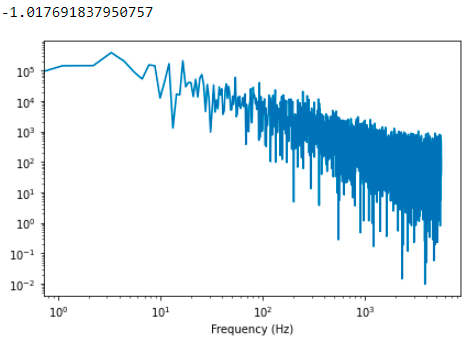
\includegraphics[width=\textwidth]{img/vvos_power.png}
                \caption{Spectrum's power plot}
                \label{fig:part5_1}
            \end{figure}
    
    \newpage
        \section{Conclusion}
            More advanced skills and knowledge of signals, waves spectrum and spectrogram was acquired. Noise - is a random unwanted modification, that affects the signal. Also noise - is signal with a lot of chaotic components, that doesn't have a harmonic structure. There are different types of noise. We've learned some of them - white, pink, red, Gaussian and Poisson. We've learned, how can we generate a noise and analyze it.
     
\end{document}
